\section{Problem (3)}

	The \cref{fig:hw9_problem3} shows an approximate plot of force magnitude $F$ versus time $t$ during the collision of a $42 \ g$ Superball with a wall. The initial velocity of the ball is $35 \ m/s$ perpendicular to the wall; It rebounds directly back with approximately the same speed, also perpendicular to the wall. What is $F_{max}$, the maximum magnitude of the force on the ball from the wall during the collision?

	\begin{figure}[H]
		\begin{center}
			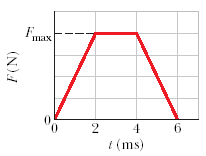
\includegraphics[scale=1]{hw9_problem3}
			\caption{Illustration of Problem 3}
			\label{fig:hw9_problem3}
		\end{center}
	\end{figure}

	\textbf{R:}

	\begin{align}
		m = \ &42 \ g \times \left(\frac{1 \ kg}{1000 \ g}\right) = 0.042 \ kg& \notag \\
		p_{i} = \ &(0.042 \ kg)(35 \ m/s)& \notag \\
		= \ &1.47 \ N \times s& \notag \\
		p_{f} \approx \ &(0.042 \ kg)(-35 \ m/s)& \notag \\
		= \ &-1.47 \ N \times s& \notag
	\end{align}
	\begin{align}
		I = \ &\Delta p = (-1.47 \ N \times s) - (1.47 \ N \times s)& \notag \\
		= \ &- 2.94 \ N \times s& \notag \\
		I = \ &F_{ave} \Delta t& \notag \\
		(-2.94 \ N \times s) = \ &F_{max} [(4 \ ms) - (2 \ ms)]& \notag \\
		F_{max} = \ &\frac{|- 2.94 \ N \times s|}{0.002 \ s}& \notag \\
		= \ &1470 \ N&
	\end{align}
